\documentclass[preprint]{sigplanconf}
\usepackage[utf8]{inputenc}

\usepackage{amsmath}
\usepackage{todonotes}
\presetkeys{todonotes}{inline}{}
\usepackage{graphicx}
\usepackage{tikz}
\usepackage{url}

\begin{document}
\conferenceinfo{FHCP '13}{23 September 2013, Boston, Massachusets, US.} 
\copyrightyear{2013} 
\copyrightdata{[to be supplied]} 

\titlebanner{Preprint, version 1.0}        % These are ignored unless
%\preprintfooter{short description of paper}   % 'preprint' option specified.

\title{A practical survey of functional GPU languages}
%\subtitle{Subtitle Text, if any}

\authorinfo{Martin Dybdal}
           {DIKU, University of Copenhagen}
           {dybber@dybber.dk}
\authorinfo{Philip L. Carlsen}
           {DIKU, University of Copenhagen}
           {plcplc@gmail.com}
\authorinfo{Ken Friis Larsen}
           {DIKU, University of Copenhagen}
           {kflarsen@diku.dk}

\maketitle

\begin{abstract}
  We present a survey of the GPU languages Accelerate
  \cite{chakravarty2011accelerating}, Nikola
  \cite{mainland2010nikola}, Copperhead \cite{Catanzaro2011}, NESL/GPU
  \cite{bergstrom2012nested} and Thrust \cite{Thrust}. We report on
  both qualitative and quantitative findings from using them in
  practice.

  We have taken two cases from the domain of computational finance and
  ported them to each of the languages, discovering limitations in the
  mean time. 

  Their performance on the two cases is compared with efficient CUDA
  implementations from the CUDA SDK.

  The aim is that the paper can be used to get an overview of the
  current state of existing GPU languages and as a ``do's and don'ts''
  for future research in this area.
\end{abstract}

% \category{CR-number}{subcategory}{third-level}

% \terms
% term1, term2

% \keywords
% keyword1, keyword2

\section{Introduction}
Graphics Processing Units (GPUs) is a cost-efficient choice for
problems with data-parallel solutions. Their massively data-parallel
architecture can deliver a high-throughput for many problems in the
sciences, engineering and finance.

Currently, OpenCL and CUDA are the most popular GPU programming
frameworks in both academia and industry. They both require manual
memory management, neither provides any means for automatic
deforestation (fusion), and they only offer little abstraction from
the underlying hardware, such that for instance, memory coalescing
must be on your mind during implementation.

To make GPU programming more accessible, quite a number of new
high-level data-parallel languages as well as GPU libraries for
existing languages have been developed \cite{Catanzaro2011,
  chakravarty2011accelerating, mainland2010nikola,
  svensson2011obsidian, bergstra2010theano, homepage:rgpu,
  bergstrom2012nested, homepage:bohrium}, though none of them have
achieved the same popularity and attention as programming directly in
OpenCL or CUDA.

In this paper we present our experience of applying a few functional
data-parallel languages to two problems from the domain of
computational finance and report on the current state of the
languages. Our scope is both qualitative in terms of the ease with
which algorithms can be formulated, optimised and debugged, as well as
quantitative in terms of execution performance.

Our first experiment involves the implementation of a
\emph{quasi-random number generator}, the Sobol sequence generator,
which is an efficient choice for numerical integration and Monte Carlo
simulation \cite{acworth1998comparison}. Our second experiment is the
implementation of an option-pricing algorithm, \emph{the binomial
  method} \cite{cox1979option}. Both of these algorithms have been
implemented in Accelerate \cite{chakravarty2011accelerating}, Nikola
\cite{mainland2010nikola}, Copperhead \cite{Catanzaro2011}, NESL/GPU
\cite{bergstrom2012nested}, Thrust \cite{Thrust} and their performance
is compared with efficient CUDA implementations.

\paragraph{Outline} In the next two sections we will introduce the two
example programs that we will use to evaluate the languages. We will
follow that up with detailing our findings from implementing the two
cases in each of the languages. After discussing the implementation
efforts, we will look at more quantitative data, in the form of
performance benchmarks.

\section{Case I: Sobol sequence generation}
\label{sec:sobol}
The first problem that we have used to evaluate the languages is a
quasi-random number generator (QRNG), namely the \emph{Sobol sequence
  generator}. QRNGs is a category of random number generators that
aims at creating samples of low discrepancy, rather than provide good
statistical randomness. QRNGs is thus in contrast with pseudo-random
number generators (PRNGs). A visual comparison of a Sobol-sequence and
a sequence generated by the popular Mersenne Twister PRNG is presented
in Figure~\ref{fig:discrepancyplot}.
\begin{figure}
  \centering
  \begin{minipage}{0.45\linewidth}
    \begin{center}
      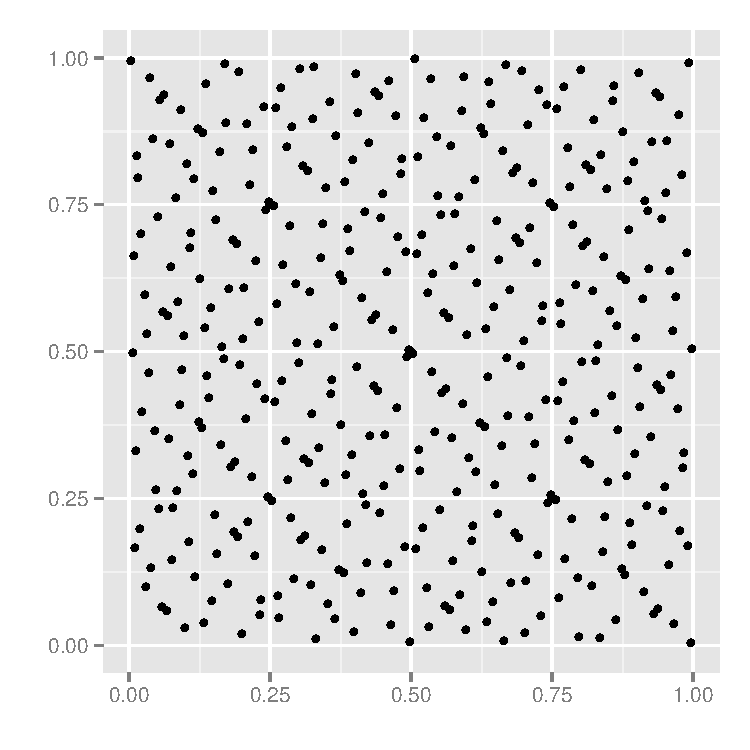
\includegraphics[width=\textwidth]{../report/graphics/2D-sobol-sequence.pdf}

      \hspace{0.55cm}\textbf{(a)}
    \end{center}
  \end{minipage}
  \begin{minipage}{0.45\linewidth}
    \begin{center}
      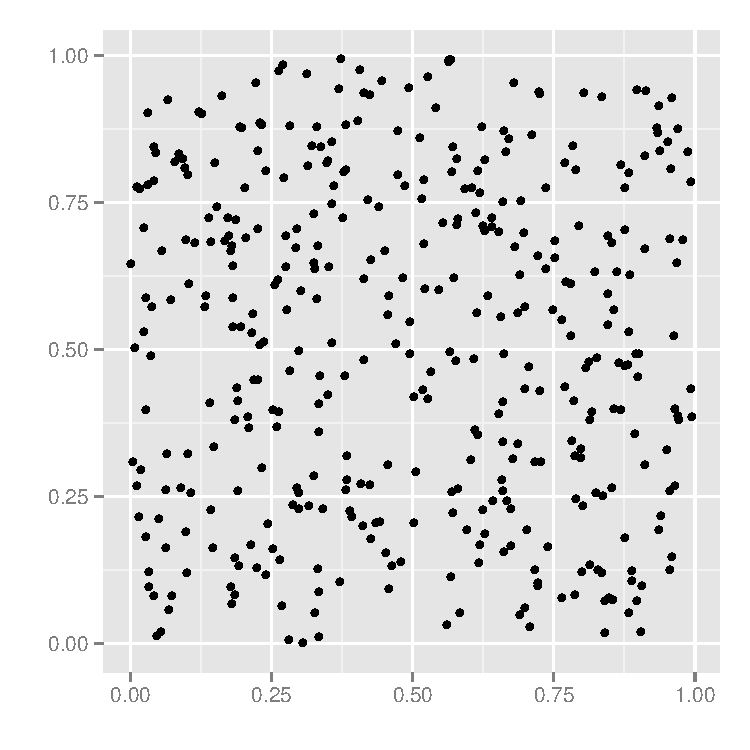
\includegraphics[width=\textwidth]{../report/graphics/2D-mersenne-sequence.pdf}

      \hspace{0.55cm}\textbf{(b)}
    \end{center}
  \end{minipage}

  \caption{\textbf{(a)} A 2D quasi-random sequence from the Sobol
    generator \textbf{(b)} A uniform 2D sequence of pseudo-random
    numbers generated with Mersenne Twister PRNG}
\label{fig:discrepancyplot}
\end{figure}
Figure~\ref{fig:discrepancyplot} illustrates that quasi-random numbers
are generated in a systematic fashion to fill out the sample space
evenly, without clusters nor holes. They are thus a poor choice for
cryptography, but in applications such as numerical integration and
Monte Carlo methods they can be efficient as they can reduce the
number of needed samples. In this case study, we use the Sobol numbers
to perform a simple $\pi$-estimation.

We will first present the implementation of an inductive formulation
of the Sobol algorithm \cite{bratley1988algorithm}, and we will later
get back to a more efficient implementation optimised for GPUs
\cite[Chapter~16]{hwy2011emerald}.

The algorithm is seeded by a so-called \emph{direction vector}. To
generate a Sobol sequence of $32$-bit numbers a direction vector of
length $32$ is required\footnote{Lists of ``good'' direction vectors are
  available online \cite{homepage:sobol:directionvectors}}. Let $v$ be
a direction vector of length $32$, the corresponding Sobol sequence is
then defined by:
\begin{equation}
x_i = v_1i_1 \oplus v_2i_2 \oplus \ldots \oplus v_{32}i_{32}\label{eq:sobol_inductive}
\end{equation}
where $i_j$ is the $j$'th bit in the binary representation of index
$i$. This sequence is then normalised to the $(0,1]$ interval.

It is not hard to translate definition~(\ref{eq:sobol_inductive}) to a
Haskell function working on lists:
\begin{verbatim}
bitVector :: Int -> [Int]
bitVector i = map (fromEnum . testBit i) [0..31]

normalise :: Int -> Float
normalise x = fromIntegral x / 2^32

sobol :: [Int] -> Int -> Float
sobol v i = normalise x_i
 where
  x_i = foldl xor 0 $ zipWith (*) v (bitVector i)
\end{verbatim}
The \verb|bitVector|-function converts the given index into its binary
representation and \verb|normalise| maps the $x_i$ integer values from
(\ref{eq:sobol_inductive}) to floating-point numbers in the $(0,1]$
interval.

To generate a complete sequence we can map over all indices:
\begin{verbatim}
sobol1D :: Word32 -> [Word32] -> [Float]
sobol1D m v = map (sobol v) [1..m]
\end{verbatim}
Higher-dimensional sequences can be generated by an additional map:
\begin{verbatim}
sobolND :: Word32 -> [[Word32]] -> [[Float]]
sobolND m vs = map (sobol1D m) vs
\end{verbatim}

In our case, where we want to compute $\pi$, we generate a
two-dimensional sequence and count how many of the coordinate-pairs
are inside and outside the unit circle. This can be done by a single
reduction operation.

% \todo{TODO: add some code that shows how to compute $\pi$, or maybe
%   it is unnecessary?}

\subsection{GPU parallelisation}
\label{sec:gpusobol}
The inductive algorithm for Sobol sequence generation is
embarrassingly parallel and can be written as a single GPU
kernel. Computing $\pi$ from a two-dimensional Sobol sequence can be
done with a parallel reduction and a post-processing step. These two
kernels can be fused together, such that the complete computation can
be executed in a single kernel without ever storing the
Sobol-sequences in GPU memory. This is what we want to achieve.

The inductive algorithm presented above requires a linear amount of
exclusive-or operations in the bit representation used for each
element of the sequence. An alternative recursive algorithm have been
shown that uses a single exclusive-or operation for each number. This
recursive algorithm have been optimised for GPUs by Thomas Bradley et
al. \cite[Chapter~16]{hwy2011emerald}. An implementation of this
GPU-optimised algorithm is included as an example in the CUDA SDK. The
algorithm progresses by first filling a block of values using the
inductive algorithm and then fill each subsequent block using a
recursive formulation from the values of the preceding iteration,
which is done by a single exclusive-or operation.

We have found it impossible to write this optimised algorithm in all
but raw CUDA, as the language lack a collective operation for building
up arrays block by block in this fashion. See Section
\ref{sec:itercons}.

\section{Case II: Binomial option pricing}
In this section we look at the problem of \emph{option pricing}. The
name \emph{option} is used collectively for a range of different
financial contracts which are time-limited opportunities to buy or
sell some underlying asset, for instance a stock. In the contract a
specific \emph{strike price} is also given, which is the pre-agreed
amount of money for buying or selling.

A particular type of options, \emph{American style options}, are
characterised by having a pre-determined constant strike price $K$,
and may be exercised in a time-interval up until the expiration time
$T$. A \emph{call option} on asset $A$ grants the right to buy $A$,
whereas a \emph{put option} grants the right to sell. For simplicity
and compatibility with the CUDA SDK implementation, we will only price
call options. We can represent this in Haskell by\footnote{We would
  normally use a record here, but records are not supported in
  Accelerate or Nikola, so we use a tuple for compatibility}.

\begin{verbatim}
type CallOption =
      ( Float -- s0   Current price of underlying
      , Float -- K    Strike price               
      , Int   -- T    Expiry in years            
      , Float -- r    Riskless interest rate     
      , Float -- vol  Volatility
      )
\end{verbatim}

To estimate the price of an American option we have to simulate the
price development of the underlying, as there is no known closed-form
analytic solution. For the simpler case of \emph{European style
  option} pricing, a closed-form solution is available in the
Black-Scholes formula \cite{black1973pricing}. 

A relatively simple discrete time model for computing the price of
\emph{American} and \emph{European style options} is the
\emph{standard binomial model}~\cite{cox1979option}.  We will use it
for pricing European options for compatibility with the CUDA SDK
implementation. The performance characteristics should map directly to
that of American option pricing.

The basic assumption is that the price of the underlying follows a
binomial process over equally spaced time steps. This makes it
possible to write out the possible future states of the
underlying. Moving a single time step forward, the binomial process
produces two possible future states of the underlying. The value of
the underlying can go either up or down with probabilities $q$ and $(1
- q)$ respectively. We denote the rate of up and down movement as $u$
and $d$ respectively. The change over one period $\Delta t$ is thus
given as:

\begin{equation}
S(t+\Delta t) = \left\{
  \begin{array}{ll}
    S(t)u & \quad \textrm{with probability $q$} \\
    S(t)d & \quad \textrm{with probability $1-q$}
  \end{array} \right.
\end{equation}

Iterating this procedure starting at time $t_0$ (now), where the
current price of the underlying is known to be $S(t_0)$, we will
obtain a binomial tree as the one in
Figure~\ref{fig:binomial-tree}. In this case we have used three
periods, the expiration time $T$ is $t_3$, and we have assumed that
$u\cdot d = 1$.

\begin{figure}
  \centering
  \tikzstyle{nodestyle} = [text centered, minimum size=0.42cm, inner sep=0]

\begin{tikzpicture}[scale=0.95, every node/.style={transform shape}]
  \node at (0,0) [nodestyle] (S1) {$S(t_0)$};

  \node at (-1, -1) [nodestyle] (dS) {$dS(t_0)$};
  \node at ( 1, -1) [nodestyle] (uS) {$uS(t_0)$};

  \node at ( 2, -2) [nodestyle] (u2S) {$u^2S(t_0)$};
  \node at ( 0, -2) [nodestyle] (S2) {$S(t_0)$};
  \node at (-2, -2) [nodestyle] (d2S) {$d^2S(t_0)$};

  \node at ( 3, -3) [nodestyle] (u3S) {$u^3S(t_0)$};
  \node at ( 1, -3) [nodestyle] (uS2) {$uS(t_0)$};
  \node at (-1, -3) [nodestyle] (dS2) {$dS(t_0)$};
  \node at (-3, -3) [nodestyle] (d3S) {$d^3S(t_0)$};

  \node at (-4.5,  0) [] (t0) {$S(t_0) =$};
  \node at (-4.5, -1) [] (t0) {$S(t_1) =$};
  \node at (-4.5, -2) [] (t0) {$S(t_2) =$};
  \node at (-4.5, -3) [] (t0) {$S(t_3) =$};

  \path[-latex]
     (S1) edge (uS)
     (S1) edge (dS)

     (uS) edge (S2)
     (dS) edge (S2)
     (uS) edge (u2S)
     (dS) edge (d2S)

     (u2S) edge (u3S)
     (u2S) edge (uS2)
     (S2)  edge (uS2)
     (S2)  edge (dS2)
     (d2S) edge (dS2)
     (d2S) edge (d3S);
\end{tikzpicture}

\vspace{2mm}

\caption{Lattice generated by the binomial process of a single
  underlying over three periods ($T=t_3$). The root node represents
  the current price of the underlying and the leafs represents
  possible values at expiration time.}
\label{fig:binomial-tree}
\end{figure}

We represent the model parameters as:
\begin{verbatim}
data BinParams = BinParams 
  { u :: Float
  , d :: Float
  , q :: Float
  }
\end{verbatim}

The main part of the program has the form:
\begin{verbatim}
binom :: Int -> Option -> Float
binom n (s0,strike,expiry,riskless,volatility) = 
   head $ foldl stepBack vFinal [1..n]
 where
   -- content of 'where'-clause is presented below
\end{verbatim}

Each step of the \verb|foldl| will discount one step backwards,
through the function \verb|stepBack|, starting at the final
$v$-values, \verb|vFinal|. \verb|vFinal| and \verb|stepBack| are
defined in the \verb|where|-clause and will be explained now.

The leaf nodes represents the possible values of the underlying at
the expiration time. After $n$ time steps, we will have $n+1$ leafs, which
values we can compute by:
\begin{verbatim}
  dt = fromIntegral expiry/fromIntegral n
  vsdt = volatility * sqrt dt
  leafs = [s0 * exp(vsdt * fromIntegral (2*i-n))
          | i <- [0..n]]
\end{verbatim}
These leafs represents all the possible prices at expiration time, and
for each possibility we can determine whether it would worthwhile to
exercise our option right:
\begin{verbatim}
  vFinal :: [Float]
  vFinal = map (\x -> max 0 $ x - strike) leafs
\end{verbatim}
From this point, we can discount backward one time-step at a time to
calculate the option price at time zero, while taking into account the
probabilities $q$ and $1-q$.
\begin{verbatim}
  rr = exp(riskless*dt)
  rrInv = 1.0 / rr
  u = exp(vsdt)         ; d = 1/u
  pu = (rr - d)/(u - d) ; pd = 1.0 - pu
  puByr = pu * rrInv    ; pdByr = pd * rrInv

  stepBack :: [Float] -> a -> [Float]
  stepBack vPrev _ = zipWith back (tail vPrev)
                                  (init vPrev)
    where back x1 x2 = puByr * x1 + pdByr * x2
\end{verbatim}

Often, we are not only interested in pricing a single option, but a
whole collection of options, a portfolio. This also enables new
opportunities for parallelisation, as we can price each option
independently. We are thus also going to examine the program:

\begin{verbatim}
binomPortfolio n options = map (binom n) options
\end{verbatim}

\subsection{GPU Parallelisation}
\label{sec:gpubinom}
We consider two simple parallelisation strategies for the binomial
option pricing algorithm. As mentioned, we are either interested in
pricing a single option, or pricing a portfolio of options.

From code of \verb|binom| above, we see that we have to synchronise
between each iteration of \verb|foldl| and the real opportunity for
parallelism in the call to \verb|zipWith| inside
\verb|stepBack|. 

Modern GPUs provides two possibilities for synchronisation. All
threads in a block/work group of threads can be synchronised by
issuing \verb|__syncthreads()| in CUDA or \verb|barrier()| in
OpenCL. Secondly, a synchronisation between all threads can happen
between each kernel invocation \footnote{In addition -- and as usually
  -- a thread synchronises with itself after each statement in its
  kernel code}.

We thus have a selection: intra-block synchronisation or inter-block
synchronisation. If we are to compute or problem in a single block, we
will be limited in the number of available threads and a single block
is expected to be mapped to a single streaming multiprocessor (NVIDIA
does not seem to define this formally).

For pricing a single option our best attempt to utilise the complete
GPU is thus to synchronise by scheduling each \verb|zipWith| as a
separate GPU kernel. For the portfolio pricer this is not a problem,
we can launch a block for each of the options to.

Other more efficient and elaborate parallelisation schemes for
binomial option pricing exists. We refer to \cite{CUDAbinomial} and
\cite{ganesan2009acceleration}.

In the next sections we will look at implementations of the above two
programs in each of the languages we have tested, and present some of
the difficulties we encountered.

\section{Accelerate}
Accelerate is a statically typed, flat data-parallel functional DSL
for array computations embedded in Haskell. Flat meaning that nested
uses of collective operations is disallowed. This limitation is
enforced by the type system.

% Accelerate is based on a set of CUDA skeletons. For each of its
% collective array operations there exist an optimised CUDA skeleton
% with a variable body,

% The parallel map in Accelerate has type:
% \begin{verbatim}
%   map :: (Shape sh, Elt a, Elt b)
%       => (Exp a -> Exp b)
%       -> Acc (Array sh a)
%       -> Acc (Array sh b)
% \end{verbatim}
% The first-order function in the first argument is written in a small
% expression language (embedded with higher-order abstract syntax),
% which is compiled into CUDA C code and inserted into the body of the
% \texttt{map}-skeleton.

% The \texttt{Exp} and \texttt{Acc} types limits how we can combine the
% different collective operations, as no \texttt{Acc} computation is
% allowed inside 

Accelerate is cleanly partitioned into front-end and back-end,
allowing for multiple backends to be developed independently. One
could imagine MPI, FPGA or OpenCL backends.

Accelerate provides no control over how operations are fused or when
data are moved between the host and device. The only way to access an
array generated by Accelerate is through a copy to host memory.

It can of course be seen as an advantage that you do not have to
manually handle data movement, but in some cases it could be desirable
to keep the data on the device and expose a raw CUDA device pointer
for further processing in another environment (e.g. an external CUDA
library).

You are not allowed to write recursive algorithms in Accelerate, if
you do, the compiler will go into an infinite loop, as it will
interpreted as an infinite program.

\subsection{Case I: Sobol sequence generation}
The type of Accelerate arrays are indexed by their dimensionality,
thus \verb|Array DIM2 Int| is a regular two dimensional array (a
matrix) of \verb|Int| values.  \verb|Vector a| is a shorthand for
\verb|Array DIM1 a|.

At first, we can translate \verb|bitVector|, \verb|normalise| and
\verb|sobol| from Section \ref{sec:sobol} more or less directly:
\begin{verbatim}
bitVectorA :: Exp Int -> Acc (Vector Int)
bitVectorA e = generate (index1 32) gen
 where gen = boolToInt . testBit e . unindex1

normaliseA :: Exp Int -> Exp Float
normaliseA x = fromIntegral x / 2.0^32

sobolA :: Acc (Vector Int) -> Exp Int -> Exp Float
sobolA v i = normaliseA (the x_i)
 where
  x_i :: Acc (Array DIM0 Int)
  x_i = fold xor 0 $ zipWith (*) v (bitVectorA i)
\end{verbatim}
The only changes is that we replace the \verb|map f [0..31]| pattern
with an application of the built-in \verb|generate|, and that we have
to use \verb|the :: Elt a => Array DIM0 a -> Exp a| to extract the
value of the singleton array returned by the \verb|fold|.

The next step becomes more complicated however, as Accelerate forbids
nested maps. Thus, we cannot write \verb|map sobolA|.  Instead we have
to push this map inside the definition of \verb|sobolA|, requiring a
manual vectorisation of both \verb|bitVectorA| and \verb|sobolA|:
\begin{verbatim}
bitVectors2D :: Exp Int -> Acc (Array DIM2 Int)
bitVectors2D n = generate (index2 n 32) gen
 where gen ix = let Z :. e :. i = unlift ix
                in  boolToInt $ testBit e i
sobol1DA :: Exp Int
         -> Acc (Vector Int)
         -> Acc (Vector Float)
sobol1DA m vec = map normalise x_i
 where
  x_i = fold xor 0 $ zipWith (*) vecRep mat
  mat = bitVectors2D m
  vecRep = replicate (lift (Z :. m :. All)) vec
\end{verbatim}
What we have done is to vectorise every operation used in
\verb|sobolA|, such that they operate on values of an additional
dimension.

If we wish to generate $n$-dimensional Sobol sequences, we will again
face the same barrier and we have to do a vectorisation in the
direction vector argument of \verb|sobol1DA|. Where we use
two-dimensional arrays we have to use three-dimensional arrays. We
will not present a \verb|sobolNDA|, but just mention that in most
parts of the sobol1DA above we would have to take the additional
dimension into account.

% \begin{verbatim}
% sobolNDA :: Acc (Array DIM2 Word32) -> Exp Int -> Acc (Array DIM2 Float)
% sobolNDA dirvs n = map normalise $ fold xor 0 $ zipWith (*) dirvs_rep (bitVectors n j)
%   where
%     j = fst . unindex2 . shape $ dirvs
%     dirvs_rep = replicate (lift $ Z :. n :. All :. All) dirvs
%     normalise x = fromIntegral x / 2^bitcount
%     bitVectors n j = generate (lift $ Z :. n :. j :. constant bitcount) helper
%       where
%         helper ix = let Z :. e :. _ :. i = unlift ix :: Z :. Exp Int :. Exp Int :. Exp Int
%                     in fromIntegral . boolToInt $ testBit e i
% \end{verbatim}

This example is a small scale illustration of a problem in languages
that disallow nested array operations. That is, flat data-parallel
languages. The fact that we could not apply \verb|sobolA| in the
context that we wanted, but had to change its inner workings showcases
a lack of composability and abstraction in such languages. When doing
the transformation, you are often forced to handle indexes manually,
re-introducing a common source of errors.

In a larger setting, the mapped function could be arbitrarily complex,
thus making the vectorisation hard to do by hand, or the function could
reside in an external library, making the transformation impossible.

It was straight forward to do the rest of the $\pi$ calculation in
Accelerate.

\subsection{Case II: Binomial option pricing}
We cannot parallelise the outer \verb|foldl| operation in
\verb|binom|, because of the dependencies between each
iteration. Thus, as previously mentioned, the parallelisation must be
found in the calls to \verb|map| and \verb|zipWith|. To do that we use
an ordinary Haskell \verb|foldl| to build up a large Accelerate
expression of repeated calls to \verb|stepBack| which will be executed
on the GPU.

An alternative parallelisation strategy is to price several options
simultaneously, a portfolio pricer, as explained in Section
\ref{sec:gpubinom}. In that case we would like to schedule the pricing
of each option as a separate thread block (work group).

\todo{explain that \texttt{syncthreads} will never be inserted, except in
  the existing skeletons, the only supported synchronization is
  by separation into independent kernels}

\begin{verbatim}
binomPortfolio n options = map (binomA n) options
\end{verbatim}

We face the same problem as in Case I: we will have to push the
\verb|map| inside the \verb|binomA| function and thus vectorise every
operation inside \verb|binomA|.

\todo{Explain that because Accelerate arrays are regular, $n$ has to
  be equal for all options, and thus $\Delta t$ will vary depending on
  the expiry time. It would be nicer if we could have constant $\Delta
  t$ and varying number of time steps for different expiry times}

% \subsection{Additional remarks} Accelerate is an active project
% with regular releases and a good online documentation. \todo{Anything
%   else?}

\section{Nikola}
Like Accelerate, Nikola is a flat data-parallel functional DSL for
array computations embedded in Haskell. Where Accelerate was based on
skeletons, Nikola is based on a small AST from which an efficient CUDA
kernel can be generated.

In contrast with Accelerate, Nikola support numerous Array types, and
it is through careful selection of these array types that fusion is
achieved. In that sense Nikola is a bit more low-level than
Accelerate. Nikola also allows for much more control of when memory
transaction occur, but can also move the arrays back and forth
automatically as necessary, if that is desired.

Nikola is very much a prototype implementation and only comes with a
few map-like higher-order operations such as: \verb|map|,
\verb|zipWith|, \verb|reshape|, \verb|generate| and \verb|replicate|,
but in contrast to Accelerate, it has a loop constructs that generates
sequential kernel code, namely \verb|iterate| and \verb|iterateWhile|.

Like Accelerate, writing a recursive program in Nikola will get the
compiler to loop infinitely.

\subsection{Case I: Sobol sequence generation}
Accelerate and Nikola turned out to have quite similar restrictions,
as they both require a flat data-parallel approach, but as mentioned,
Nikola has sequential iteration constructs, which makes this less of a
problem, as we can nest a sequential iteration inside a parallel map.

To compute $\pi$ from the 2-dimensional Sobol-sequence we need
a reduction operation, which is not included in Nikola. Nikola does
only provide a few mapping operations and a iteration construct for
sequential iteration inside a CUDA-kernel. Instead we have to use a
divide-and-conquer algorithm which requires the scheduling of
$O(lg~n)$ kernels.

\subsection{Case II: Binomial option pricing}

% \subsection{Additional remarks} Nikola does not come with much
% documentation, and you are often left to study the code, to discover
% new functionality. A tutorial is available. The project is very
% irregularly updated and is handled by a single maintainer. The
% existing research paper does not reflect the current Nikola, very much
% has changed.

\section{Copperhead}
Copperhead is a nested data-parallel functional DSL for GPU computing
embedded in Python. It is statically typed and uses Hindley-Milner
type inference, even though it is embedded inside a dynamically typed
language. Their method for mapping nested operations to GPUs is
different than flattening, as they observe the overhead incurred by
the flattening transformation. Instead, they schedule the different
layers of the program to the different layers of the parallel
architecture of a GPU (sequential code on the device, thread blocks,
grid of blocks, sequence of kernel executions).

\subsection{Case I: Sobol-sequence generation}
Copperhead does in theory support everything we need to do a direct
translation from the above Haskell code for Sobol sequence generation,
but the current implementation does not support nesting as promised in
their research paper. The interpreter returns an error if you attempt
to nest any of the collective operations.

We thus have to follow a flat data-parallel approach like we did in
Accelerate, but this turned out to be quite difficult, as the language
was designed with nesting in mind. For example, if we want to process
a two-dimensional array of type \verb|[[Int]]|, there is no way to
\verb|map| over the \verb|Int|'s of the inner arrays, as is
necessary if we want to scale all values as done in \verb|normalise|
above.

We did only complete an implementation using nested calls, which we
thus are not able to run. Writing a flat version seemed too tedious to
be worth the effort. We can thus only provide information about
Copperheads performance on Case II.

\subsection{Case II: Binomial option pricing}
In this case, no nesting was necessary, and we could thus implement
the binomial pricer without troubles:
\begin{verbatim}
@cu
def final(s0,strike,expiry,r,vol,n):
  ...
@cu
def stepBack(vPrev,expiry,r,vol,n):
  ...

def binom(s0,strike,expiry,r,vol,n):
  vFinal = final(s0,strike,expiry,r,vol,n)
  def closure(vPrev,i):
    return stepBack(vPrev,expiry,r,vol,n)
  price = reduce(closure, range(n), vFinal)
  return price[0]
\end{verbatim}

The \verb|reduce| used here is equivalent to the sequential
\verb|foldl| in Haskell. We cannot partially apply a function in
Python, therefore the named closure.

Nesting is necessary for writing the portfolio pricer, and we are thus
again unable to provide any benchmarks.

\section{Thrust}
Thrust is a C++ template library for parallel computing on GPUs (using
CUDA). The interface resembles the C++ Standard Template
Library. Thrust consist of a set of highly optimised CUDA skeletons
for parallel reduction, prefix sum, mapping, index space
transformations, sorting and searching.

Memory management is manual, but it is simplified compared to using
CUDA directly. There are two vector types, \verb|device_vector| and
\verb|host_vector|, that specifies where the data is
located. Assigning a \verb|device_vector| to a \verb|host_vector|
variable will initiate a device to host memory copy.

Fusion is partially manual. If you use a \verb|transform| or
\verb|zip| directly, fusion will not occur. Instead, you have to use
iterator versions of the collective operations that you want to fuse
together. This is made difficult by the lengthy types that you have to
use for these iterators, but the clutter can be limited by using
\verb|typedef|s and template type variables.

\subsection{Case I: Sobol-sequence generation}
In the Sobol sequence generator we had to use four different iterators
to achieve all the fusion that we wanted:
\begin{verbatim}
typedef counting_iterator<int>            Iter0;
typedef transform_iterator<sobol, Iter0>  Iter1;
typedef zip_iterator<tuple<Iter1, Iter1>> IterZip;
typedef transform_iterator<dist, IterZip> IterDist;
\end{verbatim}

\subsection{Case II: Binomial option pricing}

\section{NESL/GPU}
NESL/GPU is a GPU back-end for the parallel functional programming
language NESL \cite{nesl}. The back-end reuses the front-end of the
CPU implementation of NESL, which compiles to an intermediate language
called VCODE, which is a flattened version of the NESL
program. NESL/GPU optimises this VCODE by performing fusion where
possible and finally interpret the optimised VCODE by issuing
corresponding CUDA kernels generated during fusion.

\subsection{Case I: Sobol-sequence generation}
NESL/GPU was the most straight forward target language for our
translation of the Sobol-sequence generator. We will not include the
code here, as it is almost in one-to-one correspondence with the
Haskell code. 

A single detail is that NESL does not ship with a higher-order
reduction operation, but instead ships with a number of built-in
reductions like \verb|sum|, \verb|and|, \verb|all| and for our needs,
\verb|parity| which reduces with exclusive-or.

\subsection{Case II: Binomial option pricing}
Again, the translation was pretty straight forward. We needed a
sequential fold of \verb|stepBack| function, which we in this case was
done in a simple tail-recursive function:
\begin{verbatim}
function iter(puByr, pdByr, n, acc) =
   if n == 0 then acc
   else iter(puByr, pdByr, n-1, 
             stepBack(puByr, pdByr, acc)) $
\end{verbatim}

% \subsection{Additional remarks} Heavy system to use, as you have to
% first compile to VCODE in a Common Lisp interpreter and then optimise
% the VCODE in an SML environment, with no automatisation provided.

\section{Additional remarks}
\subsection{Iterative array construction}
\label{sec:itercons}
In neither of the languages we have found a way to implement the
GPU-optimised algorithm for Sobol-sequence construction we mentioned
in Section \ref{sec:gpusobol}. They all lack a construct for iterative
array construction. Such a construct is in Haskell known as
an \verb|unfold| function and would in Accelerate have a type similar to:

\begin{verbatim}
unfold :: Elt a => Exp Int -> (Exp Int -> a -> a)
       -> Array sh a -> Array (sh :. Int) a
\end{verbatim}
Where the first argument defines the number of times to unfold, and
the block size is defined from the size of the array argument.

\todo{Does Thrust and NESL have such an operation? \textbf{Ken:} Can't it be defined in terms of a map+scan?}


\section{Benchmarks}

\subsection{Case I: Sobol sequence generation}
\begin{figure}
  \centering
  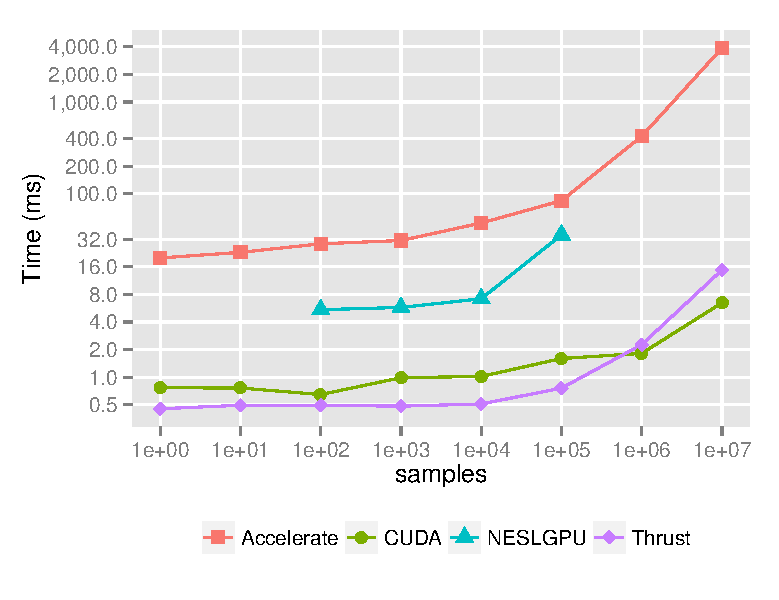
\includegraphics[width=\columnwidth]{figures/sobol-time-graph.pdf}
  \caption{Benchmark of $\pi$ calculation using Sobol sequences}
  \label{fig:bench_sobol}
\end{figure}

The CUDA SDK includes an optimised algorithm for computing
Sobol-sequences which we have extended with calls to Thrust for
computing $\pi$. Even though CUDA SDK algorithm is heavily optimised
for GPU execution, and our Thrust implementation uses the naive
inductive algorithm, we still see that Thrust outperforms it in some
cases. The problem is that we can achieve full fusion when writing
everything in Thrust, but when some parts are written in CUDA, we must
write the intermediate results to memory between kernel launches.

In the case where $n=10^5$ we see on the graph that Thrust outperforms
the CUDA SDK solution, but when inspecting with \verb|nvprof|, we
see that on raw computation CUDA SDK is still faster ($62.40 \mu s$
against $203.37\mu s$).

% CUDA, n=10^5:
%   28.417 + 16.065 + 13.089 + 4.833 = 62.404 us

% Thrust, n=10^5:
%   199.1150 + 4.25600 = 203.371 us

% CUDA, n=10^6:
%   111.05+82.12+65.25+4.54 = 262.96 us

% Thrust, n=10^6: 
%   1690 + 4.32 = 1694.32 us

% CUDA SDK, n = 100000
% ======== Profiling result:
%  Time(%)      Time   Calls       Avg       Min       Max  Name
%    41.59  111.05us       1  111.05us  111.05us  111.05us  [CUDA memcpy DtoD]
%    30.76   82.12us       1   82.12us   82.12us   82.12us  sobolGPU_kernel(unsigned int, unsigned int, unsigned int*, float*)
%    24.44   65.25us       1   65.25us   65.25us   65.25us  void thrust::detail::backend::cuda::detail::launch_closure_by_value<thrust::detail::backend::cuda::unordered_reduce_closure<thrust::transform_iterator<dist_to_origo, thrust::zip_iterator<thrust::tuple<thrust::detail::normal_iterator<thrust::device_ptr<flo
%     1.70    4.54us       1    4.54us    4.54us    4.54us  void thrust::detail::backend::cuda::detail::launch_closure_by_value<thrust::detail::backend::cuda::unordered_reduce_closure<thrust::detail::normal_iterator<thrust::device_ptr<float>>, long, float, thrust::detail::normal_iterator<thrust::device_ptr<float>>
%     0.98    2.62us       1    2.62us    2.62us    2.62us  [CUDA memcpy DtoH]
%     0.53    1.41us       1    1.41us    1.41us    1.41us  [CUDA memcpy HtoD]

% Thrust, n = 100000
% ======== Profiling result:
%  Time(%)      Time   Calls       Avg       Min       Max  Name
%                 us                us        us        us  
%    99.50  1.69e+03       1  1.69e+03  1.69e+03  1.69e+03  void thrust::detail::backend::cuda::detail::launch_closure_by_value<thrust::detail::backend::cuda::unordered_reduce_closure<thrust::transform_iterator<dist_to_origo, thrust::zip_iterator<thrust::tuple<thrust::transform_iterator<sobolInductiveFunctor, thru
%     0.25   4.32000       1   4.32000   4.32000   4.32000  void thrust::detail::backend::cuda::detail::launch_closure_by_value<thrust::detail::backend::cuda::unordered_reduce_closure<thrust::detail::normal_iterator<thrust::device_ptr<float>>, long, float, thrust::detail::normal_iterator<thrust::device_ptr<float>>
%     0.16   2.72000       1   2.72000   2.72000   2.72000  [CUDA memcpy DtoH]
%     0.08   1.40800       1   1.40800   1.40800   1.40800  [CUDA memcpy HtoD]

% CUDA, n = 10000
% ======== Profiling result:
%  Time(%)      Time   Calls       Avg       Min       Max  Name
%                 us                us        us        us  
%    42.86  28.41700       1  28.41700  28.41700  28.41700  sobolGPU_kernel(unsigned int, unsigned int, unsigned int*, float*)
%    24.23  16.06500       1  16.06500  16.06500  16.06500  [CUDA memcpy DtoD]
%    19.74  13.08900       1  13.08900  13.08900  13.08900  void thrust::detail::backend::cuda::detail::launch_closure_by_value<thrust::detail::backend::cuda::unordered_reduce_closure<thrust::transform_iterator<dist_to_origo, thrust::zip_iterator<thrust::tuple<thrust::detail::normal_iterator<thrust::device_ptr<flo
%     7.29   4.83300       1   4.83300   4.83300   4.83300  void thrust::detail::backend::cuda::detail::launch_closure_by_value<thrust::detail::backend::cuda::unordered_reduce_closure<thrust::detail::normal_iterator<thrust::device_ptr<float>>, long, float, thrust::detail::normal_iterator<thrust::device_ptr<float>>
%     3.81   2.52800       1   2.52800   2.52800   2.52800  [CUDA memcpy DtoH]
%     2.08   1.37700       1   1.37700   1.37700   1.37700  [CUDA memcpy HtoD]


% Thrust, n = 10000
% ======== Profiling result:
%  Time(%)      Time   Calls       Avg       Min       Max  Name
%                 us                us        us        us  
%    96.05  199.1150       1  199.1150  199.1150  199.1150  void thrust::detail::backend::cuda::detail::launch_closure_by_value<thrust::detail::backend::cuda::unordered_reduce_closure<thrust::transform_iterator<dist_to_origo, thrust::zip_iterator<thrust::tuple<thrust::transform_iterator<sobolInductiveFunctor, thru
%     2.05   4.25600       1   4.25600   4.25600   4.25600  void thrust::detail::backend::cuda::detail::launch_closure_by_value<thrust::detail::backend::cuda::unordered_reduce_closure<thrust::detail::normal_iterator<thrust::device_ptr<float>>, long, float, thrust::detail::normal_iterator<thrust::device_ptr<float>>
%     1.20   2.49600       1   2.49600   2.49600   2.49600  [CUDA memcpy DtoH]
%     0.69   1.44000       1   1.44000   1.44000   1.44000  [CUDA memcpy HtoD]

Accelerate is very slow on this example, the bottleneck is the Sobol
sequence generator. The part of the programming that has to do with
computing $\pi$ is just as fast as the Thrust implementation. 

In Accelerate the complete computation of \verb|sobolNDA| is fused
into a single kernel, a reduction kernel that reduces a
multidimensional array (originating from the exclusive-or
reduction). In Thrust, this is a \verb|map|-kernel, as we are able to
do the reduction sequentially (Accelerate does not provide any
primitives for sequential iteration). In the case where $n=10^5$ this
reduction takes 44.23ms, two orders of magnitude more than in
Thrust. Furthermore, because we end up with a reduction, this
computation can not be fused into the computation of $\pi$ as happened
in Thrust, so we also get a penalty for extraneous memory
transactions.

A solution would be to write the Sobol sequence generator with
completely unrolled loops, we have not attempted this, but it should
be possible in our case, as the number iterations is fixed.


% \section{Related work}
% Disposition:
% \begin{itemize}
% \item Mention some of the languages we haven't tested. See if can put
%   them in categories where the above problems are present and aren't,
%   even though we haven't tested them as much.
% \item Any similar efforts int
% \end{itemize}

\section{Future work}
We had to restrict ourselves to a few languages and only two example
cases, because of time considerations, but there are many more GPU
languages that should be considered and with the two problems we have
implemented, we only touch on a few parts of what a GPU language
should support. It would therefore be nice to extend the comparison to
cover more languages and add additional languages.

Additional languages we would have liked to include: Obsidian, Bohrium
\cite{homepage:bohrium}, Theano \cite{bergstra2010theano}, R+GPU
\cite{homepage:rgpu}, MATLAB GPU, CUB and Modern GPU.

The parallel computing group Berkeley partition problems into
equivalence classes depending on the type of computation and data
movement involved \cite{homepage:dwarfmine}, a good approach for
selecting a set of covering benchmarks would thus be to select a
problem from each of these equivalence classes. The classes include:
Dense linear algebra, sparse linear algebra, spectral methods, n-body
methods, MapReduce, graph traversal, finite state machines,
combinatorial logic, dynamic programming among others.

% Disposition;
% \begin{itemize}
% \item Extend the survey to cover additional languages:
%   Modern GPU, Bohrium, Theano, CUB
% \item Extend the survey to cover additional problems:
%   LSM, 7 dwarfs
% \item Create a larger performance benchmark of the different
%   languages
% \item Comparison of GPU-NESL VCODE and Bohrium bytecode
% can Bohrium be used as a NESL backend?
% \end{itemize}

\section{Conclusion}
* No reuse of memory in binomial option pricer

Summarise, mention GPU-NESL and other languages we haven't tested.

\acks 

We would like to thank Trevor McDonell, Lars Bergstrom, Geoffrey
Mainland, Manual Chakravary, Bryan Catanzaro and John Reppy, for first
of all making their systems readily available for all to download, and
secondly for being really quick to provide help, hints and feedback
via email, and in many cases providing quick bugfixes or workarounds.

 % \todo{for .. something about quick bugfixes, help email
 %  conversations, hints and help}


\bibliographystyle{abbrvnat}
\bibliography{../bibliography/bibliography}

\end{document}

% LocalWords:  OpenCL CUDA GPU Carlsen Dybdal Sobol Nikola QRNG QRNGs
% LocalWords:  PRNGs Mersenne PRNG dimensionality composability
% LocalWords:  vectorisation Scholes
